 %%
%%
\documentclass[12pt]{book}
\usepackage{amsfonts}
\usepackage{amsmath}
\usepackage{amssymb}
\usepackage{graphicx}
\usepackage{hyperref}
\setlength{\textheight}{10in}
\setlength{\textwidth}{7.4in}
\setlength{\topmargin}{-0.75in}
\setlength{\oddsidemargin}{-0.5in}
\setlength{\evensidemargin}{-0.5in}
\setlength{\parskip}{0.15in}
\setlength{\parindent}{0in}

\begin{document}


\vspace{-1.0in}\begin{center}
\Large{MHF4U :  Advanced Functions }

\Large{Assignment \#3}


\end{center}

%\medskip

\vspace{0.015in}\hrulefill\ 

\textbf{Reference Declaration} %  Fill in your Reference Declarations in this section before your submit your assignment.
Complete the Reference Declaration section below in order for your assigment to be graded.

If you used any references beyond the course text and lectures (such as other texts, discussions with peers or online resources), indicate this information in the space below.  If you did not use any aids, state this in the space provided. 

Be sure to cite appropriate theorems throughout your work. You may use shorthand for well-known theorems like the FT (Factor Theorem), RRT (Rational Root Theorem), etc. 

Note: Your submitted work must be \textbf{your original work}. 

Family Name: \\%Family Name Here
First Name: %First Name Here

Declared References: 

% Type your references here.
% You can use as many lines as required.

\vspace{0.015in}\hrulefill\ 

\newpage

%%%%%%%%%%%% PROBLEMS START HERE

\begin{enumerate}

%% PROBLEM 1
\item Prove the identity $\sin(x)\cos(x)=1-\dfrac{\sin^2(x)}{1+\cot(x)}-\dfrac{\cos^2(x)}{1+\tan(x)}$. Remember to use proper form for proving trigonometric identities by indicating the identities you are using.

\newpage

%% PROBLEM 2
\item Determine equivalent expressions for both of $\sin(4x)$ and $\cos(4x)$ entirely in terms of $x$. You do not need to justify your steps.


\newpage

%% PROBLEM 3
\item A circle is centered at the origin with a radius of 25. Inside this circle is an inscribed rectangle with its bottom edge on the x-axis and the two vertices on the opposite side on the circumference of the circle,. Represent the area, $A$, of the rectangle:

\begin{enumerate}
\item In terms of $x$, the distance between the y-axis and the right leg of the rectangle. 
\item In terms of $\theta$, where $\theta$ is an angle in standard position with its terminal arm on the upper right vertex of the rectangle.
\end{enumerate}

%%% You can omit the inclusion of these images from your own submission.

\begin{figure}[h]
\centering
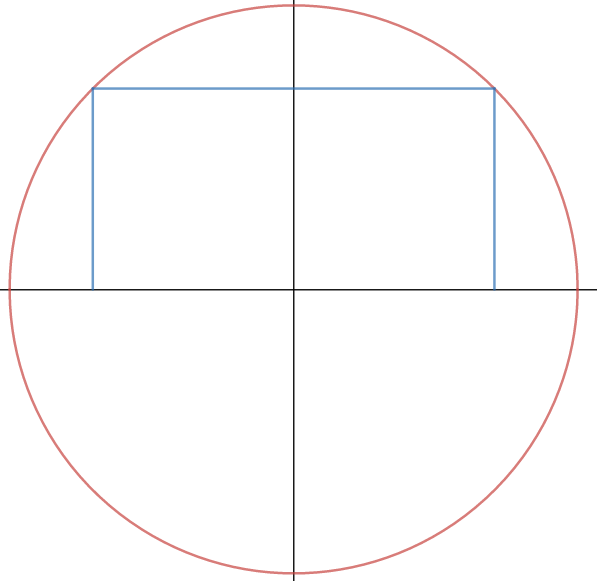
\includegraphics[scale=0.25]{Inscribed1.png}
\caption{Diagram for part a}
\end{figure}

\begin{figure}[h]
\centering
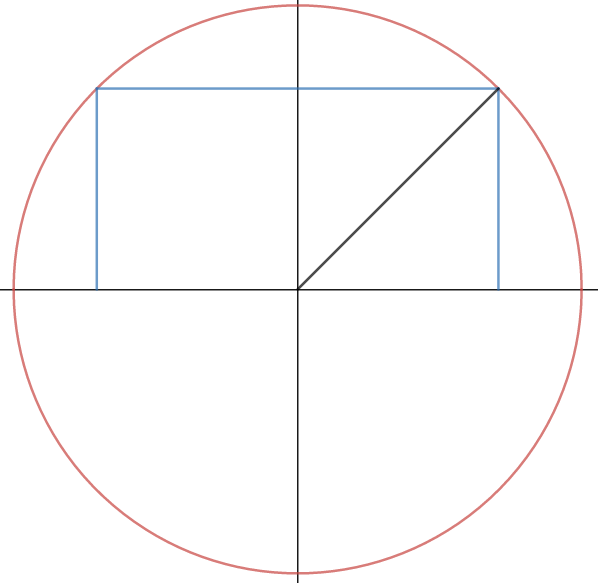
\includegraphics[scale=0.25]{Inscribed2.png}
\caption{Diagram for part b}
\end{figure}

\newpage


%% PROBLEM 4
\item Solve $2\sin^2(x) + \sin(2x) = 2$ $(x \in \mathbb{R})$. Be sure to effectively communicate the multiple solutions.


\newpage

%% PROBLEM 5
\begin{minipage}{4in}
\item Go to the website of the \href{http://worldweather.wmo.int/}{World Meteorological Organization} and select a city from the map (right).
Once you select a city, click on Climatological Information which is a tab above the map. Locate and record the data for mean max. temperature and mean min. temperature into a table. Using the data, create models for the relationship between the day of the year and both the high and low mean respectively. Finally, test the accuracy of each model by using it to determine the temperature for a single day, each.
\end{minipage}\hspace{0.2in}
\begin{minipage}{1in}
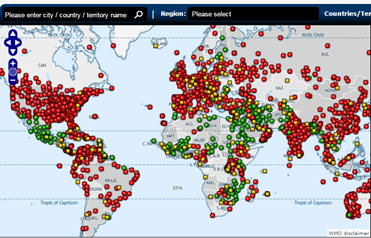
\includegraphics[scale=0.75]{WorldMap.png}
\end{minipage}

\newpage


\end{enumerate}
\end{document} 
